\documentclass[a4paper,12pt]{article}
\usepackage{amsmath}
\usepackage{amssymb}
\usepackage[polish]{babel}
\usepackage{polski}
\usepackage[utf8]{inputenc}
\usepackage{indentfirst}
\usepackage{geometry}
\usepackage{array}
\usepackage[pdftex]{color,graphicx}
\usepackage{subfigure}
\usepackage{afterpage}
\usepackage{setspace}
\usepackage{color}
\usepackage{wrapfig}
\usepackage{listings}
\usepackage{datetime}

\renewcommand{\onehalfspacing}{\setstretch{1.6}}

\geometry{tmargin=2.5cm,bmargin=2.5cm,lmargin=2.5cm,rmargin=2.5cm}
\setlength{\parindent}{1cm}
\setlength{\parskip}{0mm}

\newenvironment{lista}{
\begin{itemize}
  \setlength{\itemsep}{1pt}
  \setlength{\parskip}{0pt}
  \setlength{\parsep}{0pt}
}{\end{itemize}}

\newcommand{\linia}{\rule{\linewidth}{0.4mm}}

\definecolor{lbcolor}{rgb}{0.95,0.95,0.95}
\lstset{
    backgroundcolor=\color{lbcolor},
    tabsize=4,
  language=C++,
  captionpos=b,
  tabsize=3,
  frame=lines,
  numbers=left,
  numberstyle=\tiny,
  numbersep=5pt,
  breaklines=true,
  showstringspaces=false,
  basicstyle=\footnotesize,
  identifierstyle=\color{magenta},
  keywordstyle=\color[rgb]{0,0,1},
  commentstyle=\color{Darkgreen},
  stringstyle=\color{red}
  }

\begin{document}

\noindent
\begin{tabular}{|c|p{11cm}|c|} \hline 
Grupa 3 & Adam Nowak & \ddmmyyyydate\today \tabularnewline
\hline 
\end{tabular}


\section*{Zadanie 1 - Macierze OMP}

Opis w kilku zdaniach jak to wspaniale działa program. Wyjaśnione tutaj jest w jaki sposób udało się uzyskać równoległe działanie programu. Przytoczony poniżej fragment kodu pokazuje najważniejszy askepkt działania naszego programu.

\begin{lstlisting}
#pragma omp parallel for 
for(int i = 0; i < 10000000; i++)
{
	double * d = new double[100000]; 
	cout << "om nom nom" << endl;
}
\end{lstlisting}


Poniżej kodu znajduje się jego opis, który nie jest opisem w stylu "Tak, to nawet działa! Jest pętla i jest kolorowe. Szkoda, że się nie rusza". 

Poniżej zamieszone są wykresy na dowód posiadania umiejętności obsługi pakietu biurowego Microsoft Office Excel lub LibreOffice Calc. Można tutaj również pochawlić się znajomością małego lecz potężnego programu gnuplot.

\begin{figure}[!hbp]
	\centering
  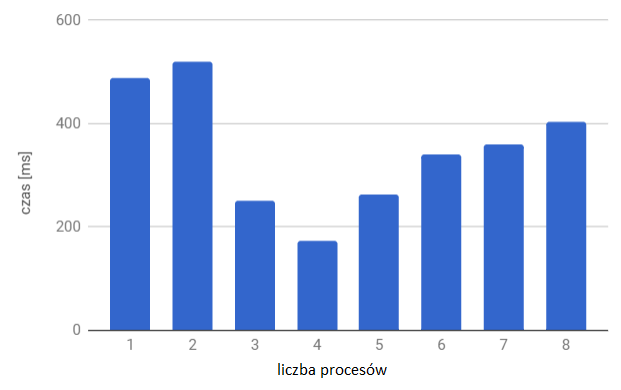
\includegraphics[width=0.7\textwidth]{dane/wykres.eps}
  \caption{Profesjonalna prosta czerwona kreska z kropkami}
\end{figure}

\begin{wrapfigure}{r}{0.5\textwidth}
  \vspace{-20pt}
  \begin{center}
  \includegraphics[width=0.45\textwidth]{dane/pomiar.pdf}
  \end{center}
  \vspace{-20pt}
  \caption{Krzywa niebieska kreska}
  \vspace{-10pt}
\end{wrapfigure}


W celu ułatwienia pracy Prowadzącemu warto wykresy podpisać, aby Prowadzący omyłkowo nie przyjął, że dany wykres przedstawia średnią miesięczną temperaturę w Bangladeszu na przełomie lat 1975-1982, ponieważ taki wykres byłby nieodpowiedni, przez co sprawozdanie byłoby niezaliczone. Łatwo zauważyć, że każdy wykres w przestrzeni 2D posiada dwie osie i z grzeczności należy je opisać. Osie posiadają jednostki, które też warto przytoczyć.

Czasem w sprawozdaniu warto przytoczyć kilka zalet danego rozwiązania i wypisać je jako lista:
\begin{lista}
 \item Pierwszą zaletą jest to, że jest.
 \item Druga zaleta jest również obecna.
 \item Trzecia zaleta jest już troche naciągana.
 \item Czwarta zaleta jest wadą, czyli zaletą ujemną.
\end{lista}

Jeśli zaszłaby konieczność zestawienia danych wartości w tabeli to również jest taka możliwość.

\begin{table}[!hbp]
\centering
\begin{tabular}{|p{5cm}|c|}
\hline 
Zalety & Wady \tabularnewline
\hline 
 Ładne, kolorowe & Brak\tabularnewline
 Szybkie, działające & Brak\tabularnewline
\hline
\end{tabular}
\caption{Podpis bardzo wartoścowej tabeli z danymi}
\end{table}


W sprawozdaniu muszą znaleźć się wnioski. Wnioski stanowią przesłankę, o tym iż osoba je pisząca, która ubiega się o tytuł magistra inżyniera, wie co robi. Osoba taka często jest w stanie określić czemu miało służyć dane ćwiczenie, a także ocenić w jakim stopniu udało się rozwiązać dane zagadnienie i gdzie napotkano problemy.

\end{document}
